In this section, we evaluate the performance of our framework. A prototype of
the framework has been implemented in the Go programming language \cite{go}.
Aspiring to a clear separation of concerns, the implementation is broken down
into of dozens of libraries, each of which is intended to be useful on its own.
The corresponding source code is available online \cite{sources}, which also
includes our experimental setup along with all configuration files and input
data. The experiments discussed below are conducted on a \up{GNU}/Linux machine
equipped with 16 processors Intel Xeon E5520 2.27~\up{GH}z and 24~\up{GB} of
\up{RAM}.

We shall get to grips with $3 \times 2 \times 3 = 18$ uncertainty-quantification
problems. There are considered three platform sizes $\np$: 2, 4, and 8
processing elements; two application sizes $\nt$: 10 and 20 tasks; and three
quantities of interest $\g$: the end-to-end delay, total energy consumption, and
maximum temperature defined in \eref{end-to-end-delay}, \eref{total-energy}, and
\eref{maximum-temperature}, respectively.

\subsection{Configuration}

A platform with $\np$ processing elements and an application with $\nt$ tasks
are generated randomly by the \up{TGFF} tool \cite{dick1998}. The tool generates
$\np$ tables and a directed acyclic graph with $\nt$ nodes. Each table
corresponds to a processing element, and it describes certain properties of the
tasks when they are mapped to that particular processing element. Namely, each
table assigns two numbers to each task: a reference execution time, chosen
uniformly between 10 and 50~ms, and a power consumption, chosen uniformly
between 5 and 25~W. The graph captures data dependencies between the tasks. The
application is scheduled using a list scheduler \cite{adam1974}. The mapping of
the application is fixed and obtained by scheduling the tasks based on their
reference execution times and assigning them to the earliest available
processing elements (a shared ready list).

The construction of thermal \up{RC} circuits needed for temperature analysis is
delegated to the HotSpot tool \cite{skadron2004}. The floorplan of each platform
is a regular grid wherein each processing element occupies $2 \times
2~\text{mm}^2$ on the die. The output of the tool is a pair of a thermal
capacitance matrix $\mC$ and a thermal conductance $\mG$ matrix used in
\eref{thermal-system}. For simplicity, the leakage modeling is based on a linear
approximation \cite{yang2013, ukhov2012, liu2007}. The time step of power and
temperature profiles is constant and equal to one microsecond; see \sref{power}
and \sref{temperature}.

\begin{figure}[t]
  \centering
  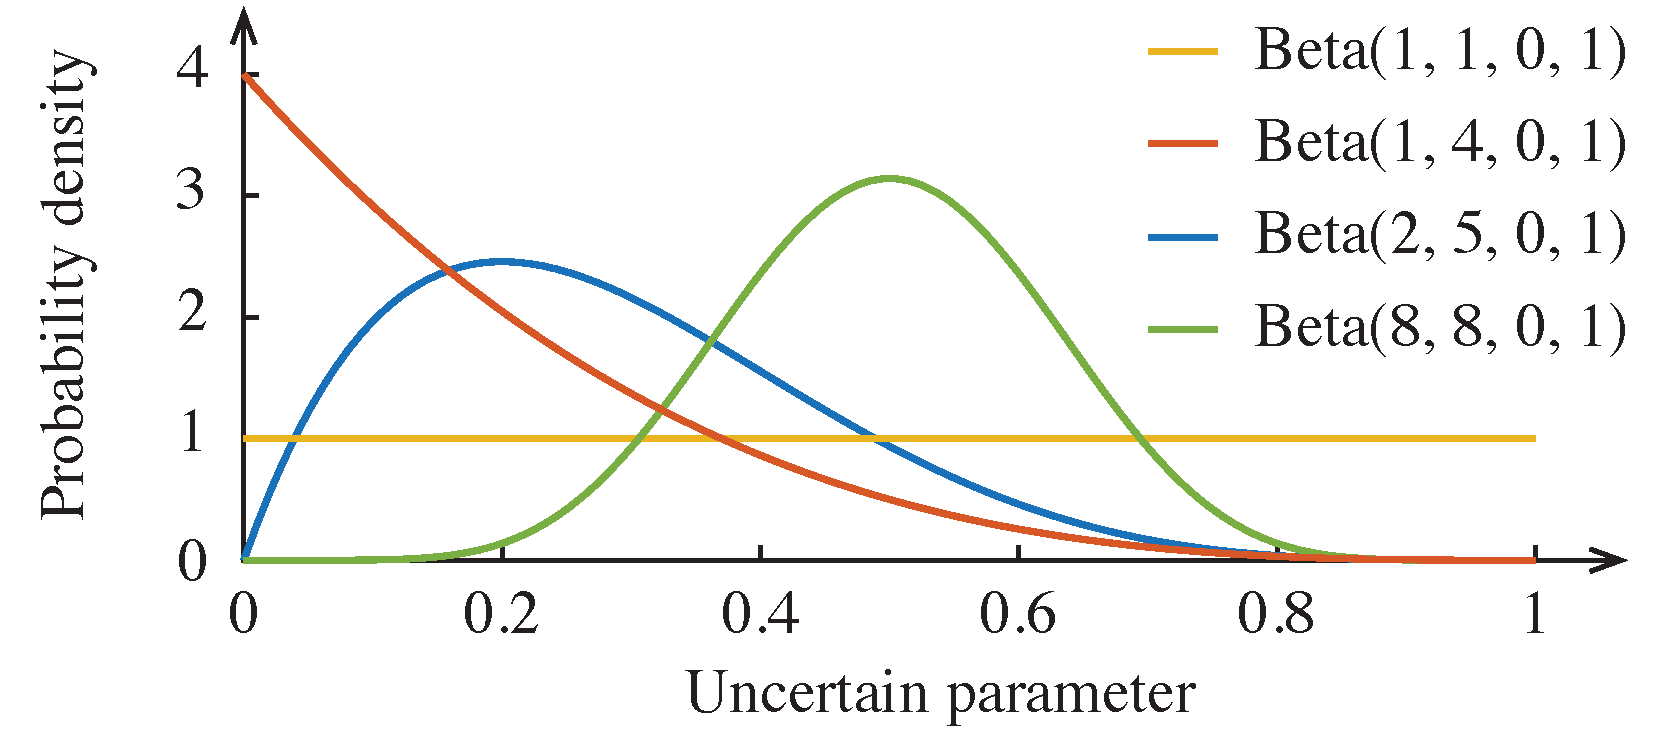
\includegraphics[width=1.0\columnwidth]{include/assets/figures/distribution.pdf}
  \caption{An illustration of the family of beta distributions.}
  \flab{distribution}
\end{figure}

The uncertain parameters $\vu$ are the execution times of the tasks; all other
parameters are deterministic. Targeting the practical scenario described in
\sref{parameters}, the marginal distributions and correlation matrix of $\vu$
are assumed to be available. Without loss of generality, the marginal of $\u_i$
is a four-parametric beta distribution $\text{Beta}(\alpha_i, \beta_i, a_i,
b_i)$ where $\alpha_i$ and $\beta_i$ are the shape parameters, and $a_i$ and
$b_i$ are the endpoints of the support. This family of distributions is very
rich; \fref{distribution} illustrates how the density function changes
dramatically depending on $\alpha_i$ and $\beta_i$. The left $a_i$ and right
$b_i$ endpoint are set to 80\% and 120\%, respectively, of the reference
execution time generated by the \up{TGFF} tool as described earlier. The
parameter $\alpha_i$ and $\beta_i$ are set to two and five, respectively, for
all tasks, which skews the corresponding distribution toward the left endpoint
as shown in \fref{distribution}. The execution times of the tasks are correlated
based on the structure of the graph produced by the \up{TGFF} tool: the closer
task $i$ and task $j$ are in the graph as measured by the number of edges
between vertex $i$ and vertex $j$, the stronger $\u_i$ and $\u_j$ are
correlated. The model-order reduction parameter $\eta$ in \eref{reduction}
(\sref{parameters}) is set to 0.9, which results in $\nz = 2$ and 3 preserved
variables for applications with $\nt = 10$ and 20 tasks, respectively.

The configuration of the interpolation algorithm (the collocation nodes, basis
functions, and adaptation strategy with stopping conditions) is as described in
\sref{interpolation}. The parameters $\aerror$, $\rerror$, and $\serror$ vary
depending on the problem and can be found at \cite{sources}, which, again,
contains all other details too.

The performance of our framework with respect to each problem is assessed as
follows. First, we obtain the ``true'' probability distribution of the quantity
in question $\g$ by sampling $\g$ directly and extensively. Direct sampling
means that $\g$ is evaluated \emph{as is}; in particular, no model-order
reduction is perform, which could affect the resulting accuracy (see
\sref{parameters}). Second, we construct an interpolant for $\g$ and estimate
$\g$'s distribution by sampling the interpolant. In both cases, we draw $10^5$
samples; let us remind, however, that the cost of sampling the interpolant is
practically negligible. Third, we perform another round of direct sampling of
$\g$, but this time we draw as many samples as many times the quantity of
interest was evaluated during the interpolation process. In each of the three
cases, the sampling is undertaken in accordance with a Sobol sequence, which is
a quasi-random low-discrepancy sequence featuring much better convergence
properties than those of the vanilla Monte-Carlo (\up{MC}) sampling
\cite{joe2008}.

As a result, we obtain three estimates of $\g$'s distribution: reference (the
one considered true), proposed (the one interpolation powered), and direct (the
one equal in terms of the number of $\g$'s evaluations to the proposed
solution). The last two are compared with the first one. For comparing the
proximity between two distributions, we use the well-known Kolmogorov--Smirnov
(\up{KS}) statistic \cite{rao2009}, which is the supremum over the distance
(pointwise) between two empirical distribution functions and, hence, is a rather
unforgiving error indicator.

\begin{figure*}
  \vspace{-1.5em}
  \centering
  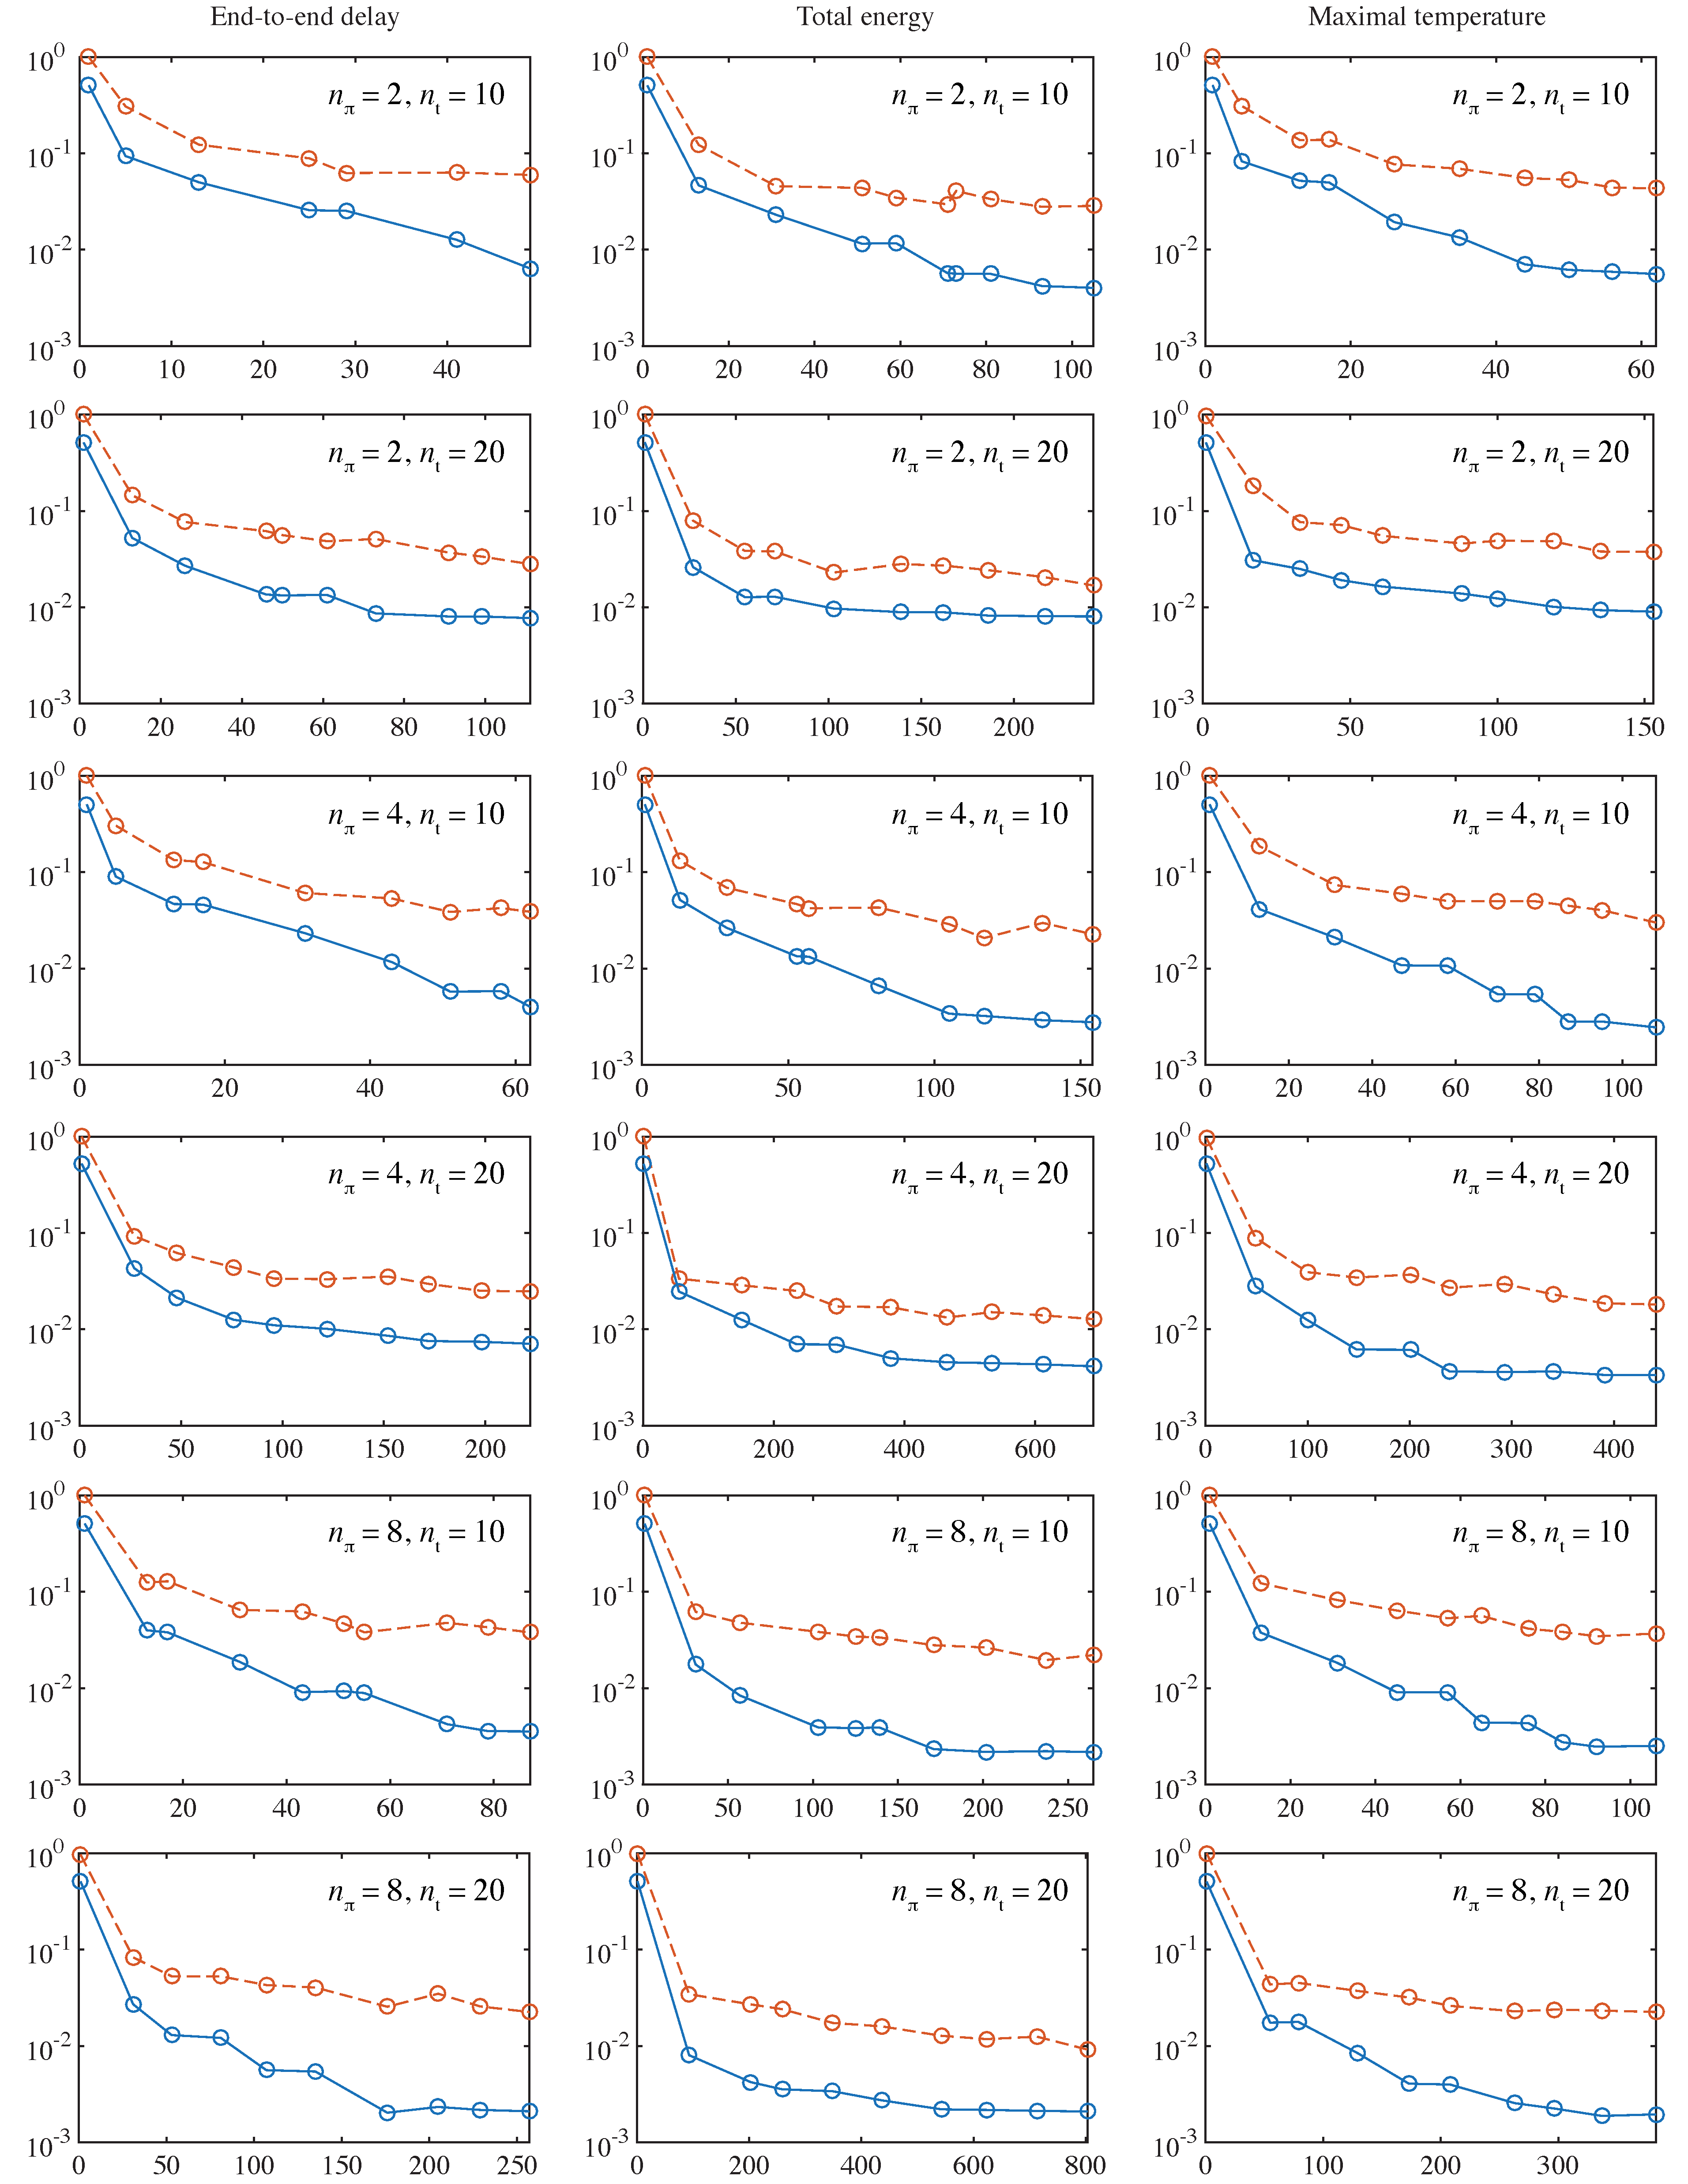
\includegraphics[width=1.0\textwidth]{include/assets/figures/results.pdf}
  \vspace{-1.5em}
  \caption{
    Experimental results. There are considered 3 platform sizes, 2 application
    sizes, and 3 quantities. The columns correspond to the three quantities: the
    end-to-end delay (left), total energy (middle), and maximum temperature
    (right). The rows alternate between the two application sizes: 10 (odd) and
    20 (even) tasks. The three pairs of rows correspond to the three platform
    sizes: 2 (top), 4 (middle), and 8 (bottom) processing elements. The
    horizontal axes show the number of points, and the vertical ones the error
    on a logarithmic scale. The solid lines correspond to our technique, and the
    dashed ones to direct sampling.
  }
  \flab{results}
\end{figure*}

\subsection{Discussion}
The results of all 18 uncertainty-quantification problems are given in
\fref{results} as a 6-by-3 grid of plots, one plot per problem. The three
columns correspond to the tree quantities of interest: the end-to-end delay
(left), total energy (middle), and maximum temperature (right). The three pairs
of rows correspond to the three platform sizes: 2 (top), 4 (middle), and 8
(bottom) processing elements. The rows alternate between the two application
sizes: 10 (odd) and 20 (even) tasks.

The horizontal axis of each plot shows the number of points, that is,
evaluations of the quantity of interest $\g$, and the vertical one shows the
\up{KS} statistic on a logarithmic scale. Each plot has two lines. The solid
line corresponds to the technique proposed in this paper. It shows how the
\up{KS} statistic computed with respect to the reference solution changes as the
interpolation process consumes more and more points, that is, as more and more
interpolation steps in \eref{approximation} are taken. Note that we display only
a subset of the actual interpolation steps in order to make the figure more
legible. Synchronously with the solid line (that is, for the same numbers of
$\g$'s evaluations), the dashed line shows the error of direct sampling, which,
as before, is computed with respect to the reference solution.

Studying \fref{results}, one can make a number of observations. First and
foremost, the interpolation-powered approach (solid lines) to probabilistic
analysis outperforms direct sampling (dashed lines) in all the cases. To
elaborate, given a fixed budget of $\g$'s evaluations, the probability
distributions delivered by our framework are closer to the true ones than those
delivered by sampling $\g$ directly, despite the fact that the latter relies on
a sophisticated sampling strategy (Sobol sequences).

The message of the above observation is that the designer of an electronic
system can benefit substantially in terms of accuracy per computation time by
switching from direct sampling to the proposed technique. If the designer's
current workhorse is the classical \up{MC} sampling, the switch might lead to
even more dramatic savings than those shown in \fref{results}. Needless to
mention that the gain is especially prominent in situations where the analysis
needs to be performed many times such as when it resides in a design-space
exploration loop.

It can also be seen in \fref{results} that the error of our technique decreases
generally steeper than the error of direct sampling. The decrease tends to
plateau toward the end of the interpolation process. This behavior can be
explained by the following two reasons. First, the algorithm has been instructed
to satiate certain accuracy requirements ($\aerror$, $\rerror$, and $\serror$),
and it reasonably does not do more than what has been requested. Second, since
the model-order reduction mechanism is enabled in the case of interpolation, the
quantity being interpolated is not $\g$, strictly speaking; it is a
lower-dimensional representation of $\g$, which already implies an information
loss. Therefore, there is a limit on the accuracy that can be achieved, which
depends on the amount of reduction applied. However, model-order reduction is a
good, recommended practice as it circumvents unnecessary complexity and,
thereby, makes problems more tractable.

At this point, it is important to realize that, for the same price, the proposed
framework yields an object that is much more rich and powerful than a bunch of
samples delivered by direct sampling. A surrogate produced by the framework for
a quantity of interest can also be used to obtain a bunch of samples, but we are
not constrained by their number. Moreover, if needed, we can always go back and
generate more samples without even touching the expansive quantity in question.
Furthermore, the placement of the collocation nodes and the magnitudes of the
corresponding surpluses are an invaluable source of information, which can be
utilized for such tasks as sensitivity analysis and edge detection. Hierarchical
surpluses are also valuable on their own; an example was given in
\sref{moments}.

Before we conclude, let us state explicitly that the wall-clock time taken by
the experiments is not reported here. This time is irrelevant: $\g$ is time
consuming (see \sref{problem}), which renders the number of $\g$'s evaluations
as the most apposite expense indicator. However, for the curious reader, we
would like to note briefly that, for instance, in the bottom-right problem shown
in \fref{results} ($\np = 8$, $\nt = 20$, and $\q$ is temperature), it took
around two hours to perform $10^5$ simulations of $\g$ in parallel on 16
processors. Evaluating the corresponding interpolant the same number of times
took less than a second.
